% =============================================================================
\section{Marcos de referencia}
% =============================================================================

\begin{frame}{Dos maneras de decir ``dónde''}
  \begin{columns}[c]
    \column{0.48\textwidth}\centering
    \textbf{Gazebo: ENU}\\[0.3em]
    \begin{tikzpicture}[scale=1.1]
      \draw[-{Stealth},thick,rojo] (0,0) -- (1.8,0) node[right,font=\scriptsize] {x = Este};
      \draw[-{Stealth},thick,verde] (0,0) -- (0,1.8) node[above,font=\scriptsize] {y = Norte};
      \draw[-{Stealth},thick,azul] (0,0) -- (-0.9,-0.7) node[below left,font=\scriptsize] {z = Arriba (hacia ti)};
      \fill (0,0) circle (1.5pt);
    \end{tikzpicture}\\
    \scriptsize Origen: el del mundo (lo decide quien hace el mundo).
    \column{0.48\textwidth}\centering
    \textbf{PX4: NED}\\[0.3em]
    \begin{tikzpicture}[scale=1.1]
      \draw[-{Stealth},thick,verde] (0,0) -- (0,1.8) node[above,font=\scriptsize] {x = Norte};
      \draw[-{Stealth},thick,rojo] (0,0) -- (1.8,0) node[right,font=\scriptsize] {y = Este};
      \draw[-{Stealth},thick,azul] (0,0) -- (0.9,-0.7) node[below right,font=\scriptsize] {z = Abajo};
      \fill (0,0) circle (1.5pt);
    \end{tikzpicture}\\
    \scriptsize Origen: \textbf{donde arrancó PX4}, no donde está el dron.
  \end{columns}
  \vspace{0.5em}
  \begin{idea}
    \small En NED \textbf{5 m arriba es $z = -5$}. Todas las alturas que mandamos a PX4 llevan signo menos.
  \end{idea}
\end{frame}

\begin{frame}{La convención de todos nuestros mundos}
  \begin{columns}[c]
    \column{0.5\textwidth}\small
    \begin{itemize}
      \item El dron aparece en \textbf{(0, 0) de Gazebo}, mirando al \textbf{norte}
        (\cmd{yaw\_deg: 90} en \cmd{spawn.yaml}).
      \item Así el origen de PX4 coincide con el del mundo y el heading arranca en 0.
      \item Pasar de uno a otro es solo cambiar el orden:
    \end{itemize}
    \[
      \begin{aligned}
        x_{\text{PX4}} &= y_{\text{Gazebo}} &&\text{(norte)}\\
        y_{\text{PX4}} &= x_{\text{Gazebo}} &&\text{(este)}\\
        z_{\text{PX4}} &= -z_{\text{Gazebo}} &&\text{(abajo)}
      \end{aligned}
    \]
    \column{0.47\textwidth}
    \begin{tikzpicture}[scale=0.8]
      \draw[gray!40,step=1] (-1,-1) grid (4,4);
      \draw[-{Stealth},thick,rojo] (0,0) -- (4.3,0) node[right,font=\tiny] {E (x Gz, y PX4)};
      \draw[-{Stealth},thick,verde] (0,0) -- (0,4.3) node[above,font=\tiny] {N (y Gz, x PX4)};
      \node[draw,circle,fill=azulclaro,inner sep=1pt,font=\tiny] at (0,0) {H};
      \fill[naranja] (3,2) circle (3pt) node[right,font=\tiny,black] {Gz (3, 2) = NED (2, 3)};
      \draw[-{Stealth},thick] (0,0.25) -- (0,0.8);
      \node[font=\tiny,left] at (0,0.6) {nariz};
    \end{tikzpicture}
  \end{columns}
\end{frame}

\begin{frame}{Ejemplo: el pilar del puente}
  \begin{columns}[c]
    \column{0.45\textwidth}
    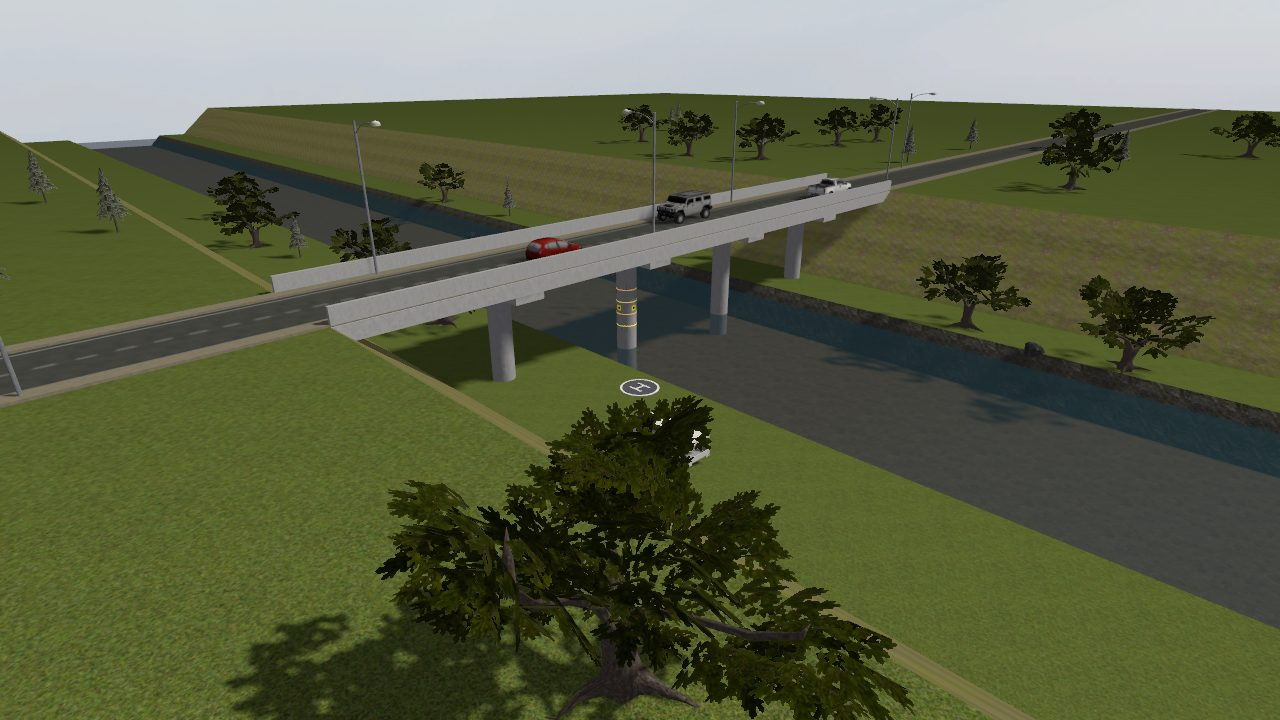
\includegraphics[width=\linewidth]{puente_rio}
    \column{0.52\textwidth}\small
    En \cmd{tools/build\_worlds.py} el pilar está en Gazebo \textbf{(6.5, 8.0)}.
    \begin{itemize}
      \item NED norte $= y_{Gz} = 8.0$ m
      \item NED este $= x_{Gz} = 6.5$ m
    \end{itemize}
    Por eso \cmd{inspeccion\_pilar} trae
    \cmd{center\_north = 8.0} y \cmd{center\_east = 6.5}.
    \vspace{0.4em}
    \begin{ojo}
      \small Si cambian de mundo o mueven el spawn, el origen de PX4 cambia y \textbf{todas}
      las coordenadas de la misión se recorren.
    \end{ojo}
  \end{columns}
\end{frame}

\begin{frame}{El marco del cuerpo: FRD}
  \begin{columns}[c]
    \column{0.45\textwidth}\centering
    \begin{tikzpicture}[scale=1.2]
      \draw[thick,fill=gray!20] (-0.5,-0.5) rectangle (0.5,0.5);
      \foreach \x/\y in {-0.7/0.7,0.7/0.7,-0.7/-0.7,0.7/-0.7} {\draw[gray] (\x,\y) circle (0.3);}
      \draw[-{Stealth},thick,verde] (0,0) -- (0,1.4) node[above,font=\scriptsize] {x: Frente};
      \draw[-{Stealth},thick,rojo] (0,0) -- (1.4,0) node[right,font=\scriptsize] {y: Derecha};
      \node[font=\scriptsize] at (0.1,-1.25) {z: Abajo (entrando)};
      \draw[-{Stealth},azul,thick] (0.55,1.0) arc (60:20:0.9) node[right,font=\scriptsize] {yaw $+$};
    \end{tikzpicture}
    \column{0.52\textwidth}\small
    \begin{itemize}
      \item PX4 describe el dron en \textbf{FRD}: x al frente, y a la derecha, z abajo.
      \item El \textbf{heading} (yaw) es el ángulo del frente medido desde el norte,
        \textbf{positivo hacia el este} (en sentido horario visto desde arriba).
      \item \cmd{vehicle\_local\_position.heading}: el yaw actual, en radianes $[-\pi, \pi]$.
      \item \cmd{vehicle\_attitude.q}: la actitud completa (roll, pitch y yaw) como cuaternión.
    \end{itemize}
  \end{columns}
\end{frame}

\begin{frame}{Del cuerpo a NED: rotar por el heading}
  \small Si el dron va nivelado, una velocidad ``adelante / derecha'' se pasa a NED así:
  \[
    \begin{pmatrix} v_N \\ v_E \end{pmatrix} =
    \begin{pmatrix} \cos\psi & -\sin\psi \\ \sin\psi & \cos\psi \end{pmatrix}
    \begin{pmatrix} v_{\text{adelante}} \\ v_{\text{derecha}} \end{pmatrix}
  \]
  \begin{columns}[c]
    \column{0.5\textwidth}
    \begin{itemize}
      \item $\psi = 0$ (mirando al norte): adelante = norte, derecha = este.
      \item $\psi = 90^\circ$ (mirando al este): adelante = este, derecha = sur.
    \end{itemize}
    \column{0.45\textwidth}
    \begin{ojo}
      \small El lidar y ROS usan \textbf{FLU} (y a la \emph{izquierda}, ángulos positivos
      a la izquierda). PX4 usa FRD. En la cueva hay que voltear signos: lo vemos ahí.
    \end{ojo}
  \end{columns}
\end{frame}

\begin{frame}{Ángulos: siempre envolver a $[-\pi, \pi]$}
  \small Restar ángulos ``a lo bruto'' falla cerca de $\pm180^\circ$:
  \[ 179° - (-179°) = 358° \quad\text{pero en realidad son } 2°. \]
  En \cmd{px4\_link.hpp}:
  \[ \text{wrap\_pi}(a) = \operatorname{atan2}(\sin a, \cos a) \in [-\pi, \pi] \]
  \begin{idea}
    \small Úsenlo cada vez que comparen dos yaws (error de apuntado en el pilar, giro hacia un hueco, etc.).
  \end{idea}
\end{frame}

\begin{frame}{De metros a GPS (y de vuelta)}
  \small Los comandos de PX4 (\cmd{DO\_REPOSITION}, \cmd{NAV\_TAKEOFF}, \cmd{DO\_SET\_HOME}) piden
  \textbf{latitud y longitud}. Para unos cuantos km basta la Tierra plana ($R = 6\,371\,000$ m):
  \[
    \text{lat} = \text{lat}_0 + \frac{\Delta N}{R}\cdot\frac{180}{\pi}
    \qquad
    \text{lon} = \text{lon}_0 + \frac{\Delta E}{R\cos(\text{lat}_0)}\cdot\frac{180}{\pi}
  \]
  \begin{itemize}
    \item Los meridianos se juntan hacia los polos: por eso el $\cos(\text{lat})$ en la longitud.
    \item Ya están hechas: \cmd{x500::gps\_offset()} y \cmd{x500::gps\_distance()}.
    \item \cmd{lat} y \cmd{lon} van en \cmd{double} (param5 y param6 del comando): en
      \cmd{float} se pierde \textasciitilde1 m.
  \end{itemize}
\end{frame}

\begin{frame}{¿Dónde está nuestro mundo en el planeta?}
  \small Todos los mundos usan la ubicación de los mundos de PX4 (Zúrich):
  \[ \text{lat}_0 = 47.397971^\circ \qquad \text{lon}_0 = 8.546164^\circ \]
  \begin{ojo}
    \small El \cmd{<magnetic\_field>} del mundo corresponde a ese lugar. Si cambian la ubicación sin
    cambiar el campo magnético, el chequeo de brújula de PX4 falla
    (\emph{``strong magnetic interference''}).
  \end{ojo}
  \vspace{0.3em}
  Ejemplo: la plataforma del barrio está 36 m al norte y 16 m al este de la farmacia
  $\Rightarrow$ lat 47.3982949, lon 8.5463757.
\end{frame}
